
\section{DBAP法を用いた音像定位}

はじめに,複数のスマートデバイスを使ってどのように音像定位するのかについて述べる.
今回のような平面配置のスピーカアレイを用いて音像定位をする手法として,
Distance-based amplitude panning (DBAP) 法\cite{dbap}がある.

DBAP法は,
任意の数のスピーカの位置が既知であり,
端末間のスピーカの出力特性が等しいとしたときに,
仮想音源と各スピーカとの距離から距離減衰を計算することで,
各スピーカの振幅を制御して音像を合成する手法である.

位置 $(x_s,y_s)$ にある仮想音源 $VS$ から,
位置 $(x_i,y_i)$ にある端末 $i$ への距離 $d_i$ を次のように定義する(図\ref{fig:DBAP}).

\begin{figure}[p]\centering
  \hspace{-2mm}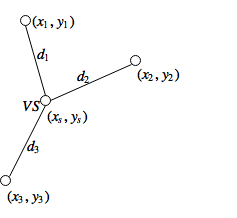
\includegraphics[clip,width=1.1\hsize]{img/DBAP.png}
  \caption{DBAP}\label{fig:DBAP}
\end{figure}

$$
d_i = \sqrt{(x_i - x_s)^2 + (y_i - y_s)^2} \qquad (\mathrm{for}\ 1 \leq i \leq N)
$$

DBAP法では,仮想想源の位置に関係なく,各スピーカからの音の強さの合計は

$$
I = \sum_{i=1}^N v_i^2 = 1
$$

として正規化している.
$i$ 番目のスピーカの相対的な振幅は距離に反比例するので

$$
v_i = \frac{k}{d_i^a}
$$

と定義できる.
$k$ はすべてのスピーカと仮想音源の位置に依存した係数で,

$$
k = \frac{1}{\sqrt{\sum_{i=1}^N \frac{1}{d_i^{2a}}}}
$$

である.
係数 $a$ は距離減衰係数で

$$
a = \frac{R}{20 \log_{10}2} \\
$$

と定義する.
$R$ はロールオフ係数で,受聴者と音源の距離に基づく減衰の量である.
$R=6\ [\mathrm{dB}]$ の場合は,
自由空間における距離減衰の逆二乗則に基づき,音の強さのレベルが音源からの距離が2倍になるごとに6dBずつ減少することを意味する.
また,半自由空間では $R=3\sim5\ [\mathrm{dB}]$ 程度となる.

以上のとおり,
複数のスマートデバイスが
同期的に制御でき,
端末の位置が判明しており,
端末間のスピーカの出力特性が均一であれば,
この手法を用いて音像定位ができることが分かった.
